Графиком функции является "галочка".

\begin{figure}[h!]
	\centering
	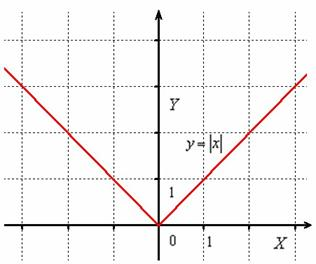
\includegraphics[width=0.5\textwidth]{img/image377.jpg}
	\caption{Функция модуля}
\end{figure}

Перепишем модуль в виде:
\begin{equation*}
    y =
    \begin{cases}
    x, \text{ если } x\geq0 \\
    -x, \text{ если } x<0 \\
    \end{cases}
\end{equation*}

Таким образом, построение сводится к построению линейных функций.

Если под модулем стоит не только x - решается аналогично. Подробнее в разделе Типовые преобразования функций.

